\documentclass[a4paper]{article} % A4 paper and 11pt font size

\usepackage{braket}
\usepackage{amsmath}
\usepackage{amssymb}
\usepackage{bm}
\usepackage[utf8]{inputenc}
\usepackage{verbatim}
\usepackage{tikz}
%\usepackage{pgfornament}
\usepackage{pgfplots}
\usepackage{pgffor}
\usepackage[version-1-compatibility]{siunitx}
\usepackage{fancyhdr}
\usepackage{lipsum}
\usepackage{gensymb}
\usepackage{framed}
\usepackage{cancel}
\usepackage{slashed}
\usepackage{hyperref}
\usepackage{pdflscape}
\usepackage{graphicx}
\usepackage{caption}
\usepackage{subcaption}
\usepackage{geometry}
\usepackage{yfonts}
\usepackage{calc}
\usepackage{cite}
\usepackage{siunitx}

\newcommand{\utilde}[1]{\tilde{#1}}

\newcommand{\vect}[1]{\mathbf{#1}} %3D vector

\setlength{\parindent}{0em}
\setlength{\parskip}{1em}
\newcommand{\goth}[1]{{\Huge\textfrak{#1}}}
\renewcommand{\baselinestretch}{1.1}

\newcommand{\exercise}[2]
{
\begin{framed}
\textbf{Exercise:} #1 \\\hrule
#2
\end{framed}
}

\newcommand{\example}[2]
{
\begin{framed}
\textbf{Example #1:} #2
\end{framed}
}

\newcommand{\review}[1]
{
\hrule
A short review:

#1
\hrule
}

\renewcommand{\picture}[1]
{
\begin{figure}[h]
\centering
\includegraphics[width=0.5\textwidth]{#1}
\end{figure}
}

\newcommand{\picturesize}[2]
{
\begin{figure}[h]
\centering
\includegraphics[width=#2\textwidth]{#1}
\end{figure}
}

\newcommand{\bmx}[1]{
\begin{bmatrix}
#1
\end{bmatrix}
}

\newcommand{\pmx}[1]{
\begin{pmatrix}
#1
\end{pmatrix}
}

\renewcommand{\tilde}{\widetilde}

 \geometry{
 a4paper,
 total={210mm,297mm},
 left=28mm,
 right=28mm,
 top=30mm,
 bottom=40mm,
 }


%----------------------------------------------------------------------------------------
%	TITLE SECTION
%----------------------------------------------------------------------------------------
%\setlength\parindent{0pt} % Removes all indentation from paragraphs - comment this line for an assignment with lots of text


\pagenumbering{arabic}
\begin{document}
\pagestyle{empty}

\newcommand{\HRule}{\rule{\linewidth}{0.5mm}}

\begin{titlepage}

    \begin{center}
        \textsc{\large SN: 587623}\\[6cm]

        \HRule \\[0.5cm]
		\Huge \textbf{PHYC90012 General Relativity}\\[0.5cm]
        \huge \textbf{Course Summary}\\[0.5cm] 
        \HRule \\[1.5cm]
        \begin{minipage}{0.4\textwidth}
        \begin{center}

        \large By \\[0.75cm]
        \huge Braden \scshape Moore \\[0.5cm]
        \normalsize \normalfont Master of Science \\
        The University of Melbourne \\

        \end{center}
        \end{minipage}

        \vfill

        \large \today
    \end{center}


\newpage
\end{titlepage}
%----------------------------------------------------------------------------------------
\pagestyle{empty}
\tableofcontents
\newpage

\pagestyle{fancy}
\pagenumbering{arabic}
\rfoot{\textsc{Braden Moore, 587623}}
\lfoot{\textsc{\today}}
\lhead{\textsc{Semester 1, 2016}}
\rhead{\textsc{PHYC90012 General Relativity}}
\setcounter{page}{1}
\setcounter{section}{-1}
\section{Syllabus}
\subsection{Part I}
\begin{enumerate}
\item Introduction to gravity
\begin{itemize}
\item Order of magnitude estimates
\item Small amount of quantum gravity
\end{itemize}
\item Equivalence principle
\item Experimental foundations
\item Geometric objects
\begin{itemize}
\item Need to understand geometric components of GR
\item Vectors, metric, etc. that live on manifolds
\item Laws of nature do not depend on coordinates chosen
\item Hence can write laws of nature in terms of geometric objects w/o reference to coordinates
\end{itemize}
\item Kinematics
\begin{itemize}
\item Time dilation, length contraction in GR framework
\end{itemize}
\item Calculus in curvilinear coordinates
\begin{itemize}
\item Mass and energy curve space time
\item Hence geometric objects moved on curved manifolds
\item Distances are not only spatial but temporal; need to use mathematics of small change = calculus
\item Uses the covariant derivative (a geometric object; independent of basis/coordinate independent)
\item This point of the course we will not be considering curved space, but instead only curvilinear coords 
\begin{itemize}
\item A flat space can be covered (represented?) by curved coordinates, but an intrinsically curved surface cannot be covered by flat coordinates
\end{itemize}
\end{itemize}
\item Curved spaces
\begin{itemize}
\item Manifolds 
\item How to calculate lengths, volumes, angles in curved spaces
\item Introduces the idea of parallel transport $\Rightarrow$ leads to curvature
\item Define the Riemann tensor, and its children etc. Ricci tensor, ...; these satisfy the Bianchi identities
\end{itemize}
\item Einstein's field equations
\begin{itemize}
\item Stress-energy tensor
\end{itemize}
\item Weak-field limit
\begin{itemize}
\item Gauge transformations
\end{itemize}
\subsection{Part II - Applications}
\item GR phenomena revisited 
\begin{itemize}
\item GPS, Mercury's orbit, gravitational lensing, gravitational redshift, ...
\end{itemize}
\item Gravitational waves
\begin{itemize}
\item Propagation (phase speed, polarisation, ...)
\item Generation*
\item Detection*
\begin{itemize}
\item[*] = together these form the ``antenna problem"
\end{itemize}
\end{itemize}
\item Relativistic stars
\begin{itemize}
\item neutron stars
\item equation of state (cannot study on Earth because largest nuclei only have 200 elements or so; need more density)
\end{itemize}
\item Black holes
\begin{itemize}
\item Event horizons, singularities, ...
\end{itemize}
\item Cosmology
\begin{itemize}
\item Friedman-Robertson-Walker (FRW) metric - describes a homogeneous, isotropic universe
\begin{itemize}
\item We will derive this and the Friedman equations
\end{itemize}
\end{itemize}

\end{enumerate}


\section{Introduction to gravity}
\subsection{Strength of gravity}
\begin{itemize}
\item Weak! Weakest of all fundamental forces
\item Long-ranged force (like EM)
\item Weakness determined by coupling constant
\item Coupling constant = Newton's gravitational constant
\end{itemize}
\begin{equation}
\vec{F}=\frac{Gm_1 m_2}{r_{12}^2}\hat{r}
\end{equation}
\begin{itemize}
\item G is hard to measure; least well known of coupling constants
\end{itemize}
In 1797-98, Cavendish used torsion balls (1.8m torsion balance) with rod of big masses and rod of small masses. 
\begin{itemize}
\item Spring constant of torsion balance was measured from free oscillation
\item then introduced 158kg balls
\item measured deflection angle of balance $\Rightarrow$ can calculate force
\begin{itemize}
\item using a mini-telescope against Vernier scale
\end{itemize}
\item rearrange Newton's law to get G
\end{itemize}

\picture{images/cavendish-torsion-balance.png}
 
\exercise{Show that Cavendish also measured density of Earth as a bonus at the same time.}
{Mass of Earth $M_{\oplus}= \rho V$ where $V=\frac{4}{3}\pi R^3$ assuming the Earth is a sphere. How does calculating $G$ also calculate $\rho$? Well, we have $\vec{F}=\frac{Gm_1 m_2}{r_{12}^2}\hat{r}$. Let's take $m_1 = M_\oplus$ as the mass of the Earth, and $m_2 = m$ as some small object mass. Let's imagine the smaller object falling to the center of the Earth. We'll take $r_{12}$ as the distance from the object to the Earth's center, which we can approximate as Earth's radius, i.e. $r_{12}=R$. This force should be equivalent to $F=ma$.\\
\\
So we have
\begin{align*}
\frac{GM_\oplus m}{R^2}&=mg\\
\frac{G\rho \frac{4}{3}\pi R^3}{R^2}&=g\\
\frac{4G \rho \pi R}{3}&=g\\
\Rightarrow \rho &=\frac{3g}{4\pi GR}\\
&=\frac{3\times \SI{9.8}{ms^{-2}}}{4\pi\times \SI{6.67384d-11}{\kg^{-1}\m^3 \s^{-2}}\times \SI{6370}{km}}\\
&=\frac{3\times 9.8}{4\pi\times 6.67384\times 10^{-11}\times 6370\times 10^3}\si{\kg.m^{-3}}\\
&=\SI{5503}{kg.m^{-3}}
\end{align*}
}


\begin{itemize}
\item Modern $G=6.67384(80)\times \SI{d-11}{Nm^{-2}.\kg^{-2}}=\si{\kg^{-1}.\m^3.\s^{-2}}$
\item Product GM is known to 1 part in $\sim 10^{10}$ from astrophysics observations
\begin{itemize}
\item[$\Rightarrow$] mass is hard to measure gravitationally
\end{itemize}
\item We need a dimensionless number to characterise strength
\item Newton: $\Phi=\frac{GM}{r}$ (potential)
\item In free fall: $\frac{KE}{mass}$, $v^2 \sim \frac{GM}{r}$
\item We claim gravity is strong is free-fall is relativistic, i.e. $v\sim c$
\item This is an order of magnitude estimate
\end{itemize}


\subsection{Strong vs. weak gravity}
\begin{itemize}
\item Quasi-Newtonian:
\begin{itemize}
\item characteristic speed of body in free fall: $v^2\sim \frac{GM}{r}$
\end{itemize}
\item Strong gravity leads to relativistic free fall, i.e. $\frac{GM}{Rc^2}\geq 1$ where M is the total mass and R is th characteristic size
\end{itemize}

\begin{table}
\centering
\begin{tabular}{c|cc} 
 & $\frac{GM}{Rc^2} \lll 1$ & $\frac{GM}{Rc^2}\geq 1$\\
\hline $v \ll c$ & Newtonian & CAN'T EXIST \\
$v\sim c$ & special rel. & full GR (difficult)
\end{tabular}
\end{table}

\example{1.1}{
$M=M_{\odot}$ (mass of the Sun)
\begin{align*}
R & \sim \frac{GM}{c^2} \text{\quad boundary of strong regime}\\
&\sim \frac{10^{-10}10^{30}}{10^{17}}\\
&\sim \text{km}
\end{align*}
cf. Schwarz radius of black hole $=\frac{2GM}{c^2}$
}
\example{1.2}{
Density of black hole with mass of $M_\odot$
\begin{align*}
&\sim \frac{M}{R^3}\sim\frac{\SI{d30}{kg}}{\si{(km)^3}}\\
&\sim 10^{21}kgm^{-3}
\end{align*}
How does this density compare to maximum density of (say) nuclear matter? Let's compare.
\begin{align*}
\frac{m_n}{(1fm)^3}\sim \frac{10^{-27}kg}{10^{-45}m^3}\sim 10^{18}kgm^{-3}
\end{align*}
We see a black hole is more dense that a nuclei. The characteristic size of a particle $1fm\sim\Delta x\sim \frac{\hbar}{\Delta p}\sim \frac{\hbar}{m_n c}$, due to Heisenberg's uncertainty principle, and also the Pauli exclusion principle.
}
More generally: density of material that forms black hole $\sim\frac{M}{R^3}$, but note $M=\frac{c^2R}{G}$ density $\rho \propto \frac{1}{R^2}$. This means that denser black holes are smaller.

\exercise{Estimate the strength of gravity $\frac{GM}{Rc^2}$ on Earth.}

\example{2}
{
The Universe is composed of 5\% baryons + 25\% dark matter + 70\% dark energy. Estimate M and R.\\\hrule
$R\sim \SI{10}{Gpc}$
\begin{itemize}
\item Mass of baryons 
\begin{itemize}
\item $10^{11}$ stars in Milky Way
\item $(10^4)^3$ galaxies in Universe
\item[$\Rightarrow$] $M_{\text{baryons}}\sim10^{23}M_\odot\sim \SI{d53}{kg}$
\end{itemize}
\end{itemize} 
\begin{equation}
\frac{GM_{tot}}{Rc^2}\sim\frac{10^{-10}\cdot 10^{53}\cdot 10}{10^{27} \cdot 10^{17}}\sim 1
\end{equation}
\begin{align*}
\text{Density }\rho\sim\frac{M_{tot}}{R_{tot}^3}&\sim\frac{c^2}{R^2G}\text{, use }\frac{GM}{Rc^2}\sim 1\\
&\sim\frac{1}{G\times(\text{age of universe})^2}
\end{align*}
cf. critical density from Friedmann equations $\rho_{crit}=\frac{3H_0^2}{8\pi G}$.\\
Recall Hubble constant $H_0\sim \frac{1}{\text{age}}$.
}
The critical density is the density of the universe at which expansion will asymptotically slow. Too dense leads to big crunch, too low leads to unbounded expansion.
\exercise{How do we reconcile a ``flat" universe from critical density with the ``curved" universe?}

Important to remember: gravity is strong when $\frac{GM}{Rc^2}\sim 1$, which occurs around black holes, the universe at large. In a sense, cosmological results such as critical density, expansion of universe come from this.

\subsection{Black hole oscillations}
We can estimate the oscillation frequency of a ``black hole'' (i.e. something with $\frac{GM}{Rc^2}\sim 1$ as $\sim \frac{c}{R}$; that is, the time is takes light to travel the distance of the object. This is the natural frequency for this object. Using that ubiquitous expression we can express the oscillation frequency as $\sim \frac{c^3}{GM}$, e.g. $M=M_\odot \Rightarrow \text{frequency}\sim\SI{10}{kHz}$.

Let's discuss charged black holes. It is difficult to astrophysically have charged black holes, because stars are not usually charged (due to the strength of the EM force, which would attract opposite charge and cancel out). So, these are artificial in nature. These have unusual geometry, and are called ``Reissner-Nordstrom'' black holes.
\example{}{What is the maximum charge on a black hole?\\\hrule
\begin{align*}
\frac{Q^2}{4\pi\epsilon_0 R}&\leq \frac{GM^2}{R}\\
Q&\leq (4\pi\epsilon_0 G)^{1/2} M
\end{align*}
Above, we relate Coloumb force to gravitational force. The gravitational force holding a black hole together must overcome the Coloumb force pushing it apart.
}

\subsection{Quantum Gravity}
The problem with quantum gravity is that there is no theory... hence we must rely on numerology.

We consider a hypothetical elementary excitation of a ``black hole'' (again, we mean a \emph{relativistic compact object}) of mass $M$. Hence the characteristic size, or ``wavelength'', of the excitation is $\frac{GM}{c^2}$ (fundamental excitation only). Introducing quantum mechanics: the Heisenberg uncertainty principle tells us that the zero-point motion associated with this excitation is
\begin{equation}
\lambda\sim\frac{\hbar}{\Delta p}\sim \underbrace{\frac{\hbar}{Mc}}_{\text{relativistic}}
\end{equation}
Equating length scales $\Rightarrow M_{pl}\approx \left(\frac{\hbar c}{G}\right)^{1/2}$; this is the Planck mass, about $\SI{d-8}{kg}$ (the mass below which quantum gravity is important. 

Given $M_{pl}$ we get $\lambda\sim\frac{\hbar}{M_{pl}c}\sim \SI{d-33}{m}$; the Planck length - the length where quantum gravity is important (e.g. just after Big Bang).

\subsubsection{Hawking Radiation}
Let's return to our elementary excitation with $\lambda\sim\frac{GM}{c^2}$, i.e. frequency $\sim \frac{c^3}{GM}=\frac{c}{\lambda}$. Heisenberg tells us there is an associated energy fluctuation $\Delta E\sim h\times\text{frequency}\sim\frac{\hbar c^3}{GM}$. Suppose (note: this is a huge leap) energy fluctuation in the black hole system is in thermal equilibrium with a bath at temperature $T$. Then $T\sim\frac{\Delta E}{k_B}$. This associates a temperature to a black hole.

We call a black hole a blackbody! 
\begin{align*}
\text{Radiated power }&= k_B\times \text{area} \times T^4\\
&=\sigma\times \underbrace{R^2}_{\left(\frac{GM}{c^2}\right)^2}\times \left(\frac{\hbar c^3}{GMk_b}\right)^4\\
&\propto M^{-2}
\end{align*}

\exercise{Plug in numbers to this!}{}

This shows that a black hole radiates energy $\Rightarrow$ eventually a black hole evaporates. We can estimate the time scale of this evaporation.
\begin{equation}
\text{time scale}\sim\frac{Mc^2}{\text{power}}\propto M^3
\end{equation}
$\Rightarrow$ small black holes evaporate fast!

As an aside, we could consider the rate of energy accretion. For system outside a black hole with uniform density $\rho_{\text{out}}$, we have
\begin{align*}
\text{rate of mass accretion}&\sim \rho_\text{out}\cdot c \cdot 4\pi R^2\\
\text{rate of energy accretion}&\sim c^2\cdot \text{rate of mass accretion}
\end{align*}
\hrule
A short review:
\begin{itemize}
\item there is no theory of quantum gravity
\item we consider a relativistic elementary oscillation $\lambda\sim\frac{GM}{c^2}$
\item we use Heisenberg to relate this to an energy fluctuation in the system
\item energy fluctuation can be converted to a temperature $T_H=\frac{\hbar c^3}{GMk_B}$, the Hawking temperature
\item we find small block holes evaporate more quickly than large black holes
\end{itemize}

\hrule

\subsection{Black hole thermodynamics}
\textbf{1st law}: $dS=\frac{dQ}{T}$\quad system constant volume

Hawking radiation: we lose a bit of heat $dQ$ due to blackbody radiation.
\begin{equation}
dS=\frac{GMk_b}{\hbar c^3} d(Mc^2)
\end{equation}
We see heat loss comes from rest energy
\begin{equation}
\frac{dS}{k_B}\approx \frac{1}{R^2_{\text{Planck}}}\underbrace{d(R^2)}_{R\sim\frac{GM}{c^2}}
\end{equation}
This result relates the entropy of a black hole to its area; Bekenstein-Hawking entropy - $S_{\text{black hole}}\propto\text{area of event horizon}$.
\begin{equation}
\frac{S}{k_B}=\frac{\text{area}}{4R^2_{\text{Planck}}}\footnote{In 1995, Maldacena also got this by counting microstates}
\end{equation}

However, there is a contradiction! Hawking radiation implies that $dA<0 \Rightarrow dS<0$.... this is bad.\footnote{See Ted Jacobson's lecture at University of Utrecht for a discussion on this.} One way to resolve this is by making a generalised \textbf{2nd law}:
\begin{equation}
d\left(S_{\text{outside}}+\frac{\text{area}}{4R_{\text{Planck}}^2}\right)\geq 0
\end{equation}
Unfortunately this is not enough - there is still a contradiction. Consider a small box of radiation which we prepare far from a black hole. $S_{\text{box}}=\frac{4U_{\text{box}}}{3T_\text{box}}$. We can make photons very long wavelength, so that $U_{\text{box}}\approx 0$ but $S_{\text{box}}\neq 0$. Then $dS_{\text{out}}=-S_{\text{box}}<0$. $d(\text{area})=0$ because energy in box $=0$, i.e. $d(Mc^2)=0$.\footnote{Beware the Unruh radiation.}

\exercise{Resolve the box paradox!}{}

\textbf{3rd law of BH thermodynamics}: can't reduce $T$ to zero.\footnote{If you are curious: Verlinde, 
\href{arXiv.org/abs/1001.0785}{arXiv:1001.0785}, \emph{On the Origin of Gravity and the Laws of Newton}, in which the idea of emph{gravity is an entropic force} is discussed.}

In heating a rubber band, it shrinks; this is because a shrunken arrangement of the molecules is a state of more entropy (more disordered)

\begin{center}
{
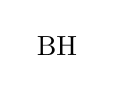
\begin{tikzpicture}
\node at (0,0) {BH};
\end{tikzpicture}
}
\end{center}

																					
\section{Einstein equivalence principle}
We will define this (the weak and strong equivalence principles), and some of the tests been performed.

\subsection{Weak equivalence principle}
Trajectory of body in free fall is independent of its mass and $\underbrace{\text{composition}}_{\text{binding energy}}$ (as per Galileo, feather vs. brick). Note that this is not equivalent for electric fields (the movement of a charged particle through an electric field depends on its charge).

\subsection{Strong equivalence principle}
\begin{enumerate}
\item weak equivalence principle is valid
\item results of any non-gravitational (e.g. EM, \underline{not} Cavendish expt) experiment is independent of velocity of freely falling frame
\begin{itemize}
\item this is \emph{local Lorentz invariance}
\end{itemize}
\item results of non-gravitational experimental are independent of where and when it is performed
\begin{itemize}
\item this is \emph{local position invariance}
\end{itemize}
\end{enumerate}

The Einstein equivalence principle (EEP) $\equiv$ strong implies: existence of a ``curved spacetime'' with:
\begin{enumerate}
\item[\textbf{i.}] symmetric metric
\item[\textbf{ii}.] trajectories of free-falling bodies are geodesics of metric
\item[\textbf{iii.}] the laws of physics in a freely-falling frame can be written in the language of special relativity
\end{enumerate}


\review{
Einstein equivalence principle:
\begin{enumerate}
\item universality of free fall
\item local Lorentz invariance
\item local position invariance
\end{enumerate}
Implications:
\begin{enumerate}
\item[3)] $\Rightarrow$ fundamental constant independent of $\vec{x}$, $t$
\item[2)] $\Rightarrow$ laws of non-gravitational physics \underline{locally} independent of frame
\item[1)] $\Rightarrow$ space is \underline{curved}
\end{enumerate}

Why is space curved? Locally straight trajectory in free yet \underline{yet} gravity produces curved trajectory (observed) $\Rightarrow$ only possible if coordinates change from one point to next
}

\section{Experimental tests}
\subsection{Experimental tests of free fall}
Inertial mass $m_i=\frac{\text{applied non-gravitational force}}{\text{measured acceleration}}$

Gravitational mass $m_g=$ ``passive'' mass appearing in weight

Look for $m_i \neq m_g$

Write 
\begin{equation}
m_g=m_i + \sum_{\text{interactions A in body}}\eta^A \frac{E^A}{c^2}
\end{equation} 
Here $E=$ ``binding energy''/potential energy of interaction $A$.

\underline{Tests:}
\begin{enumerate}
\item E{\"o}tv{\"o}s-type torsion balance experiments: two different materials may fall at difference rates (see Dicke, Braginsky)
\item Colorado: U, Cu laser interferometer $\Rightarrow relativite acceleration$
\item E{\"o}t-Wash experiments: fancy version of 1)
\end{enumerate}

Result:
\begin{equation}
\frac{|m_g-m_i|}{m_i}\leq 10^{-13}
\end{equation}

We test this, for example, with aluminium (Al) and gold (Au) weights on a torsion balance. As the Sun moves from one side of the Earth to the other, if the gravitational mass of either differs from the other we will see diurnal oscillation in the balance.

\picture{images/eotvos.png}

\subsection{Tests of local Lorentz invariance}
\begin{itemize}
\item Michelson-Morley experiment (the aether)
\item Rossi-Hall tests for lifetime of muons (time dilation $\Leftrightarrow$ LLI)
\item Ives-Stiwell transverse Doppler shift
\begin{itemize}
\item laser travelling some vector $\vec{v}$
\item we see perpendicular wave vector $\vec{k}$
\item measure frequency when laser intersects line of sight
\item Doppler shift arises due to time dilation
\end{itemize}
\end{itemize}

Mathematically:
\begin{equation}
\bmx{\omega'/c\\k'_x\\k'_y\\k'_z}=
\bmx{
\gamma&\gamma v/c&0&0\\
\gamma v/c&\gamma&0&0\\
0&0&1&0\\
0&0&0&1
}
\bmx{
\omega/c\\0\\k_y\\0
}=
\bmx{
\gamma\omega/c\\
\gamma\omega v^2/c\\
k_y\\
0
}
\end{equation}

\exercise{Compare with standard longitudinal Doppler:
\begin{equation}
\pmx{\\\text{same}\\\text{matrix}\\\\}\pmx{\omega/c\\k_x\\0\\0}
\end{equation}
}
{}

\review{Last lecture:
\begin{itemize}
\item tests of LPI
\item Schiff's thought experiment (gravitational redshift)
\end{itemize}
}

\subsection{Gravitational redshift}
\begin{equation}
\frac{h\nu'-h\nu}{h\nu}=\frac{(m_A g_A - m_B g_B)H}{(m_A-m_B)c^2}
\end{equation}
If $g_A=g_B$ (universal free-fall), then gravitational redshift is $gH/c^2$

\subsection{Observation of GR in experiments}
There are situations where GR makes measurable difference \underline{today}

\begin{itemize}
\item Pound-Rebka experiment (gravitational redshift, also seen on white dwarf spectral lines)
\item GPS
\item 2015 discovery of gravitational waves from binary BH merger
\item cosmological measurements (CMB, redshifts, $H_0$, \ldots)
\item gravitational lensing (light bent by a mass) (see: Einstein cross, Abell clusters, stars behind Sun)
\item precession of perihelion of Mercury
\item orbital decay of Hulse-Taylor binary pulsar (can calculate to mm precision the decay of the orbit every 8 hours due to gravitational wave emission)
\item Nordtredt/lunar ranging experiments
\item Gravity Probe B - lense-thinning precession
\item Shapiro time delay
\end{itemize}

\begin{figure}[h]
\centering
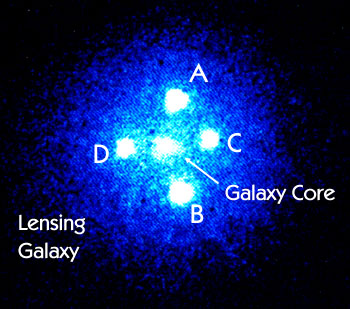
\includegraphics[width=0.5\textwidth]{images/einstein-cross.jpg}
\caption{Einstein cross}
\end{figure}


\subsubsection{Pound-Rebka experiment}
Looks at gravitational redshift of $\SI{14.4}{keV}$ gamma rays from $^{57}$Fe decay

$^{57}$Fe decays and emits photons directly down from a $\SI{23}{m}$ tall tower, to another box of $^{57}$Fe below. Gravitational redshift occurs; time moves slower closer to the Earth, so gamma ray emitted will have a different energy than that required to be absorbed by the $^{57}$Fe at the bottom.

Receiver box moves up/down at speed $v$. We adjust $v$ at bottom so that kinematic Doppler shift $\propto \left(\frac{1-v/c}{1+v/c}\right)^{1/2}$ exactly cancels the gravitational redshift $\propto gH/c^2$

N.B.: recoil (in a random direction) when photon emitted/absorbed; energy $E_R=\frac{E_\gamma}{2M_{Fe}c^2}$

\begin{equation}
E_R\sim\frac{\SI{14.4}{keV}}{\SI{100}{GeV}}\sim 10^{-7}
\end{equation}

We solve this problem through the Mossbauer effect: use whole crystal; whole crystal ($\sim10^{23}$ Fe atoms) recoils

\begin{figure}[h]
\centering
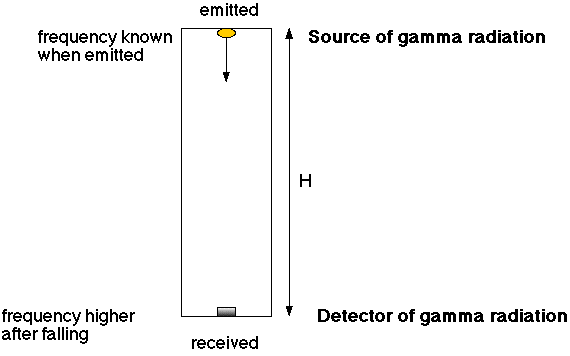
\includegraphics[width=0.5\textwidth]{images/pound-rebka.png}
\caption{Pound-Rebka experiment}
\end{figure}


\subsubsection{Lunar ranging}
Williams + Dickey (2002)\footnote{See also ``Living Reviews'' Relativity}

Moon not completely dormant
\begin{itemize}
\item fluid core (?)
\item tidal dissipation internally
\item etc \ldots
\end{itemize}

Multiple radar reflectors to improve accuracy. We search for an accurate Earth-Moon orbit versus time; we find
\begin{equation}
\frac{1}{G}\frac{dG}{dt}=(0.0\pm 1.1)\times \SI{d-12}{yr^{-1}}
\end{equation}

Uncertainty $\approx 0.02 H_0$ - we don't see increasing separation between Earth and Moon due to expansion of universe. This is expected, however: gravitational bound objects do not separate with time, although the energy they require to stay bound will increase

\subsubsection{Deflection of light (gravitational lensing)}
In a three-body system with the Earth, the Sun and another star, the light from the star will bend due to the Sun before it reaches Earth (not taking a straight path). This causes the apparent position of the star to be different than the actual position.

Deflection angle $\delta\theta \propto \frac{GM}{c^2d}$

GR deflection = $2\times$ Newtonian deflection (Einstein 1911). 

This effect is achromatic!

\subsubsection{Shapiro delay}
Roundtrip time from Earth to a distant mirror (in a three-body system including the Sun) is longer than if the Sun was not there.
\begin{equation}
\delta t\propto \frac{GM}{c^3}\ln(\text{geometric factors})
\end{equation}

Best measurements with Cassinin spacecraft (accuracy 1 in $10^5$)

\section{Geometric Objects}

\subsection{Vectors}
Invariants are measurable. Therefore, each coordinate representation is as valid as the other!

\subsubsection{Definitions of a vector}
Vector $\vec{A}$
\begin{itemize}
\item four numbers that are projections onto spacetime (can be dependent or independent of a metric)
\begin{itemize}
\item Note: vectors can have meaning without a metric
\end{itemize}
\item a geometric object with ``length'' (requires a metric) and a ``direction'', i.e. an arrow
\item a geometric object which transforms from one coordinate system to another
\item a linear function which takes a 1-form as an argument and returns a real number
\end{itemize}

$\underbrace{\text{Vector spaces}}_{\text{vectors}}\supseteq \underbrace{\text{normed vector spaces}}_{\text{length}} \supseteq \underbrace{\text{inner product spaces}}_{\text{angle}}$

$\Rightarrow$ you can have vector spaces without a norm or angle concept.

\exercise{$\vec{\Delta}x=$ displacement (in spacetime), is a vector}{}

Vector components, $A^0,A^1,A^2,A^3$; in another frame we have $A^{0'},A^{1'},A^{2'},A^{3'}$.

\subsubsection{What is a basis vector?}
Projection requires a metric (for a dot product)!
$\Rightarrow$ we have 4, special, linearly independent vectors which ``point along'' (no concept of length/angle) axes of coordinate system, $\left\{\vec{e}_{\alpha}\right\}$

\begin{equation}
\vec{A}=A^0 \vec{e}_{0} +A^{1}\vec{e}_{1}+A^{2}\vec{e}_{2}+A^{3}\vec{e}_{3} \label{vector projection}
\end{equation}

As $\vec{e}_{0}$ is itself a vector, using \ref{vector projection}
\begin{equation}
\vec{e}_{0}=(\vec{e}_{0})^{0}\vec{e}_{0}+(\vec{e}_{0})^{1}\vec{e}_{1}+(\vec{e}_{0})^{2}\vec{e}_{2}
+\underbrace{(\vec{e}_{0})^{3}}_{\text{3rd component of }\vec{e}_{0}}\vec{e}_{3}
\end{equation}

By linear independence, as $\vec{e}_0$ is linearly independent to $\vec{e}_{1},\vec{e}_{2},\vec{e}_{3}$
\begin{equation}
\Rightarrow (\vec{e}_{0})^{1}=(\vec{e}_{0})^{2}=(\vec{e}_{0})^{3}=0
\end{equation}
\begin{equation}
\Rightarrow (\vec{e}_{\alpha})^{\beta}=\delta_{\alpha}^{\beta}
\end{equation}
which is \emph{true in all coordinate systems}. Therefore in a primed frame,
\begin{equation}
\Rightarrow (\vec{e}_{\alpha'})^{\beta'}=\delta_{\alpha'}^{\beta'}
\end{equation}

\underline{But} $(\vec{e}_{\alpha'})^{\beta}\neq \delta^{\beta}_{\alpha'}$
\begin{itemize}
\item $\vec{e}_{\alpha'}$ is tied to the prime frame
\item the geometric object is only defined with respect to the frame (where $\vec{A}$ could exist in all frames)
\item you cannot measure a basis vector in another coordinate frame. You have to be in the coordinate frame to measure it.
\end{itemize}

\subsubsection{Transformations}
In general,
\begin{align*}
\left\{x^{\beta'}\right\}&\mapsto \left\{x^{\alpha}\right\}\\
\text{from }\sigma' &\to \sigma\quad\text{primed to unprimed}
\end{align*}

\begin{equation}
\Lambda^{\alpha}_{\beta'}=\frac{\partial (x^{0},x^{1},x^{2},x^{3})}{\partial (x^{0'},x^{1'},x^{2'},x^{3'})}
=\frac{\partial x^{\alpha}}{x^{\beta'}}\quad \text{16 elements!}
\end{equation}

If the transform is linear (e.g. Lorentz transform), we can consider
\begin{equation}
x^{\alpha}=\Lambda^{\alpha}_{\beta'}x^{\beta'}
\end{equation}
where $\Lambda^{\alpha}$ is not necessarily a constant. But if the transform is non-linear, the left side is wrong. We instead have
\begin{equation}
dx^{\alpha}=\Lambda^{\alpha}_{\beta'}~dx^{\beta'}
\end{equation}

Why? If we define $\vec{x}$ as a displacement from origin to the point in a curved space, there are multiple different path. We would need more than 4 numbers to define this, therefor we no longer have a meaningful vector. 

Vectors are defined localling an tangent space, \textbf{and} transformations of vectors are also restricted locally to tangent space. If $\vec{A}$ is a vector,
\begin{equation}
A^{\alpha}=\Lambda^{\alpha}_{\beta'}A^{\beta'}
\end{equation}

\review{\textbf{Vectors}

$\vec{A}$: defined in tangent space

Components $A^\alpha$: $\vec{A}=A^\alpha \vec{e}_{\alpha}$ where $\vec{e}_{\alpha}$ are basis vectors. These (unprimed) basis vectors only have meaning in unprimed coordinates

Transform like infinitesimal displacements:
\begin{equation}
\underbrace{A^{\alpha'}}_{\text{primed}}=\overbrace{\frac{\partial x^{\alpha'}}{\partial x^{\alpha}}}^{\text{transform matrix}}\underbrace{A^{\alpha}}_{\text{unprimed}}\label{vector transform}
\end{equation}

How do basis vectors transform?
\begin{align*}
A^{\alpha}\vec{e}_\alpha=\vec{A}&=A^{\alpha'}\vec{e}_{\alpha'}\\
&=\frac{\partial x^{\alpha'}}{\partial x^{\beta}}A^{\beta}\vec{e}_{\alpha'}	\\
&=\frac{\partial x^{\alpha'}}{\partial x^{\alpha}}A^{\alpha}\vec{e}_{\alpha'}
\end{align*}

This has to be true for all $\vec{A}$, i.e.
\begin{equation}
\vec{e}_{\alpha}=\frac{\partial x^{\alpha'}}{\partial x^{\alpha}}\vec{e}_{\alpha'}
\end{equation}
Or equivalently,
\begin{equation}
\vec{e}_{\alpha'}=\frac{\partial x^{\alpha}}{\partial x^{\alpha'}}\vec{e}_{\alpha}
\end{equation}
Note this is the opposite of transformation law for vector components \ref{vector transform}

\exercise{Try for Lorentz transformations.}{}
\exercise{(later) Try for 2 types of Schwarz black hole coordinates.}{}

}

\subsection{1-forms}
$\widetilde{p}$
\begin{itemize}
\item four numbers associated to four dimensions and associated to vectors in a specific way (see below)
\item geometric object that transforms like a \underline{gradient}
\item tensor of type $\pmx{0\\1}$, i.e. linear function which accepts vector as an argument and returns a real number
\end{itemize}
If we have a metric, a neat way to visualise a 1-form is as a contour.

e.g. vector is an arrow (length, direction)

cf. 1-form is contours

\picturesize{images/contour.png}{0.3}
Value of $\widetilde{p}(\vec{A})=4$; number of times $\vec{A}$ pierces surfaces of $\widetilde{p}$

Components defined to be
\begin{align*}
p_\alpha&=\widetilde{p}(\vec{e}_{\alpha})\\
&=\langle{\tilde{p},\vec{e}_{\alpha}}\rangle
\end{align*}
From lines 1 to 2, we have equivalent notation. We are using an inner product. By convention we use a lowered index.

We cannot have curved contours, as they are only defined in tangent space.

We have a neat way to calculate the coordinate-independent quantity $\tilde{p}(\vec{A})$
\begin{align*}
\tilde{p}(\vec{A})&=\tilde{p}(A^{\alpha}\vec{e}_{\alpha})\\
&=A^{\alpha}\tilde{p}(\vec{e}_{\alpha})\quad\text{linear}\\
&=A^{\alpha}p_{\alpha}
\end{align*}

This is a contraction. It is an inner product but \underline{not} dot product (we require a metric, and for it to be between two vectors, for a dot product).

Vectors and 1-forms are ``apples and oranges'' - completely different geometric objects which cannot be compared even at the same point, e.g. $\tilde{p}=\vec{A}$ is meaningless.

This is comparable to bras and kets in quantum mechanics; they form a dual space, but we cannot directly compare the objects of a pair

\subsubsection{How do 1-forms transform?}
We start with basis vectors
\begin{equation}
\vec{e}_{\alpha}=\frac{\partial x^{\alpha'}}{\partial x^{\alpha}}\vec{e}_{\alpha'}
\end{equation}
In component form:
\begin{align*}
p_{\alpha'}&=\tilde{p}(\vec{e}_{\alpha'})\\
&=\frac{\partial x^{\alpha}}{\partial x^{\alpha'}}\tilde{p}(\vec{e}_{\alpha})\quad\text{linear}\\
&=\frac{\partial x^{\alpha}}{\partial x^{\alpha'}}p_{\alpha}
\end{align*}
i.e. components of $\tilde{p}$ transform like basis vectors (\underline{not} components of basis vectors)

\review{Last lecture missing

1-forms and their relation to gradients defined
}

\subsection{1-forms, basis 1-forms and gradients}

\begin{table}
\centering
\begin{tabular}{l  | c | c}
\renewcommand\arraystretch{1}
& \textbf{Vectors} & \textbf{1-forms}\\
\renewcommand\arraystretch{2}
& $\vec{A}=A^{\alpha}\vec{e}_{\alpha}$&$p_{\alpha}=\tilde{p}(\vec{e}_{\alpha})$\\
\hline Transformation for coordinates & 
$A^{\alpha'}=\dfrac{\partial x^{\alpha'}}{\partial x^{\alpha}}A^{\alpha}$ &
$p_{\alpha'}=\dfrac{\partial x_{\alpha'}}{\partial x_{\alpha}}p_{\alpha}$ \\
\hline Transformation for basis vectors &
$\vec{e}_{\alpha'}=\dfrac{\partial x_{\alpha'}}{\partial x_{\alpha}}\vec{e}_{\alpha}$ &
$\tilde{\omega}^{\alpha'}=\dfrac{\partial x^{\alpha'}}{\partial x^{\alpha}}\tilde{\omega}^{\alpha}$
\end{tabular}
\end{table}

\review{Given a scalar field $\phi(\vec{x})$ we define a 1-form $\tilde{d\phi}$, with components $(\tilde{d\phi})_{\alpha}=\frac{\partial\phi}{\partial x^{\alpha}}$

\textbf{Notes:}
\begin{enumerate}
\item If we take $\phi$ = one of the coordinates, e.g. $\phi=x^{\alpha}$ for a specific $\alpha$, then $\tilde{d\phi}=\delta^{\alpha}_{\beta}$ for $\phi=x^{\alpha}$
\begin{itemize}
\item i.e. $\tilde{d \phi}$, for $\phi=x^{\alpha}$ is just $\tilde{\omega}^{\alpha}$, the basis 1-form
\end{itemize}
\item $\tilde{d\phi}$ is the most natural definition of a normal in GR. We also has $\tilde{d\phi}(\vec{t})=0$ if $\vec{t}$ is a tangent vector to the level surfaces of $\phi$; don't need a metric
\item How do we construct components of vectors?
\begin{itemize}
\item Components of 1-forms: $p_{\alpha}=\tilde{p}(\vec{e}_{\alpha})$
\item Dual: components of vectors: $A^{\alpha}=\vec{A}(\tilde{\omega}^{\alpha})$
\item Note that we do not need 1-forms to define vectors (and vice versa), but once we start discussing components, we do need them
\end{itemize}
\end{enumerate}
}

\subsection{Tensors}
$\pmx{M\\N}$ tensor is a linear function operating on M 1-forms and N vectors to return a real number. 

For example if $R$ is a $\pmx{1\\1}$ tensor then its components are $R^{\alpha}_{\beta}=R(\tilde{\omega}^{\alpha},\vec{e}_{\beta})$.

You can build big tensors out of little ones in several ways (and vice versa, e.g. via contraction). One important way is the outer product; 

e.g. outer product of vectors $\vec{A}$ and $\vec{B}=\pmx{2\\0}$ tensor; $T=\vec{A}\otimes \vec{B}$

Takes two 1-forms as arguments: $T(\tilde{p},\tilde{q}) \equiv^{\text{def}}\vec{A}(\tilde{p})\vec{B}(\tilde{q})$ (this is multiplying two scalar numbers)

\begin{itemize}
\item Note: outer product not commutative.
\begin{equation}
\text{If } S=\vec{B}\otimes \vec{A} \text{ then } S(\tilde{p},\tilde{q})=\vec{B}(\tilde{p})\vec{A}(\tilde{q})\neq T(\tilde{p},\tilde{q})
\end{equation}
\item Can't write a general $\pmx{M\\N}$ tensor as an outer product necessarily, but can write as a linear combination of outer products
\begin{equation}
\underbrace{T}_{\text{geometric object}}=T^{\alpha_{1},\ldots,\alpha_{M}}_{\beta_{1},\ldots,\beta_{N}}\vec{e}_{\alpha_{1}}\otimes\ldots\otimes \vec{e}_{\alpha_{M}}\otimes \tilde{\omega}^{\beta_{1}}\otimes\ldots\otimes\tilde{\omega}^{\beta_{N}}
\end{equation}
\item even though we use M 1-forms and N vectors, we take the outer product over N 1-forms and M vectors
\end{itemize}

\exercise{Show that you get the components of $T$ when you evaluate $T$ for $M$ basis 1-forms and $N$ basis vectors.}{}

Another way to generate new tensors:
\begin{align*}
\text{Symmetric part of T ($T^{(\alpha\beta)}$): }& T_{\text{(sym)}}^{(\tilde{p},\tilde{q})}=\frac{1}{2}T(\tilde{p},\tilde{q})+\frac{1}{2}T(\tilde{q},\tilde{p})\\
\text{Antisymmetric part of T ($T^{[\alpha\beta]}$): }& T_{\text{(sym)}}^{(\tilde{p},\tilde{q})}=\frac{1}{2}T(\tilde{p},\tilde{q})-\frac{1}{2}T(\tilde{q},\tilde{p})\\
\end{align*}

This example is for $\pmx{2\\0}$ but can generalise to $\pmx{M\\N}$

\subsubsection{Metric tensor}
$\pmx{0\\2}$ tensor which accepts two vectors and returns a number which we call scalar or dot product.

\begin{equation}
g(\vec{A},\vec{B})\equiv^{def}\vec{A}\cdot \vec{B}\qquad\text{this is \underline{not} contraction}
\end{equation}

Clearly bilinear

What is g? Anything we like! It depends on the coordinates we choose to use! (And it tells us how lengths, angles, $\ldots$ are measured in our favourite coordinates)

Components: 
\begin{equation}
g_{\alpha\beta}=g(\vec{e}_{\alpha},\vec{e}_{\beta})=\vec{e}_{\alpha}\cdot \vec{e}_{\beta}
\end{equation}
i.e. 16 numbers saying how the basis vectors relate to each other in any given coordinate system

What is $g(\Delta\vec{x},\Delta\vec{x})$ ($\Delta\vec{x}$ is a displacement vector)?
\begin{align*}
g(\Delta\vec{x},\Delta\vec{x})&=g(\Delta x^{\alpha}\vec{e}_{\alpha},\Delta x^{\beta}\vec{e}_{\beta})\\
&=g_{\alpha\beta}\Delta x^{\alpha}\Delta x^{\beta} \qquad\text{linear}
\end{align*}

This quantity is the spacetime interval in curved space. Invariant!

\review{Metric: $\pmx{0\\2}$ tensor $g(\vec{A},\vec{B}\equiv \vec{A}\cdot\vec{B}$

Components: 
\begin{equation}
g_{\alpha\beta}=g(\vec{e}_{\alpha},\vec{e}_{\beta})=\vec{e}_{\alpha}\cdot \vec{e}_{\beta}
\end{equation}
}

e.g. Minkowski metric
\begin{equation}
\{g_{\alpha\beta}\}=\text{diag}(-1,1,1,1)
\end{equation}
e.g. Schwarzschild black hole of mass $M$ (we will prove this later)
\thinmuskip=5mu
\begin{equation}
\{g_{\alpha\beta}\}=\left[-\left(1-\frac{2M}{r}\right),\left(1-\frac{2M}{r}\right)^{-1},~r^2,~r^2\sin^2\theta\right]
\end{equation}
where $r$ is the radial coordinate.

Vectors $\vec{A}$ and $\vec{B}$ are orthogonal vectors if $g(\vec{A},\vec{B})=0$. But orthogonal doesn't necessarily mean perpendicular.

These include 4D vectors of ``zero length'':
\begin{itemize}
\item in Minkowski, momentum of photon $\vec{p}=\left(\frac{E}{c},\utilde{p}\right)$ in flat space,
and we know $E=|\underbar{p}|c$ so $g(\vec{p},\vec{p})=-\frac{E^2}{c^2}+|\underbar{p}|^2=0$.
\begin{itemize}
\item i.e. $\vec{p}$ is orthogonal with itself; has zero ``length'' but obviously \underline{not} a zero vector, nor is it perpendicular to itself
\end{itemize}
\item in Minkowski: boost between frames
\picturesize{images/minkowski_boost.png}{0.4}
\begin{itemize}
\item the boost vectors are not perpendicular, but we still have $\vec{e}_{0'}\cdot\vec{e}_{1'}=0$
\end{itemize}
\end{itemize}


\subsection{Correspondence between vectors and 1-forms}

Let $g$ be a metric, and let $\vec{V}$ be an arbitrary vector. Then $g(\vec{V},...)$ has one argument free, and that argument is a vector, so $g(\vec{V},...)$ must be a 1-form. We call it $\tilde{V}$ because it's the 1-form associated with $\vec{V}$. What are its components?

\begin{align*}
V_{\alpha}\equiv^{def}\tilde{V}(\vec{e}_{\alpha})&=g(\vec{V},\vec{e}_{\alpha})\\
&=g(V^{\beta}\vec{e}_{\beta},\vec{e}_{\alpha})\\
&=V^{\beta}g(\vec{e}_{\beta},\vec{e}_{\alpha})\quad\text{by linearity}\\
&=V^{\beta}g_{\beta\alpha}\quad\text{by definition}
\end{align*}
This is the ``lowering the index'' operation of yesteryear! The old language for this is: lower a contravariant index, get a covariant index.

This can go the other way as long as $g$ is invertible. \underline{Define} $g^{\alpha\beta}$ as 16 numbers you get if you treat $g_{\alpha\beta}$ as a matrix and invert it.
\begin{equation}
\text{i.e.,}\quad g^{\alpha\beta}g_{\beta\gamma}=\delta^{\alpha}_{\gamma}
\end{equation}

\exercise{What is the geometric object whose components are $g^{\alpha\beta}$? Hint: $\pmx{2\\0}$ tensor which takes two 1-forms as arguments.}{}

We check that ``raising the index'' on $V_{\alpha}$ gets us back to $\vec{V}$.
\begin{equation}
V_{\alpha}\underbrace{g^{\alpha\gamma}}_{\text{inverse metric}}=
V^{\beta}g_{\beta\alpha}g^{\alpha\beta}=V^{\beta}\delta_{\beta}^{\gamma}
=V^{\gamma}
\end{equation}

More generally:
\begin{align*}
g&\text{ maps } \pmx{M\\N}\text{ tensor to }\pmx{M-1\\N+1}\text{ tensor}\\
g^{-1}&\text{ maps } \pmx{M\\N}\text{ tensor to }\pmx{M+1\\N-1}\text{ tensor}
\end{align*}

Physics example: consider a photon in curved (Schwarzschild) spacetime. 

We know $\vec{p}\cdot\vec{p}=0$ in the local freely falling frame(from weeks 1,2: Michelson-Morley experiment), and $\vec{p}\cdot\vec{p}$ is invariant $\Rightarrow \vec{p}\cdot\vec{p}=0$ in all coordinate systems. 

In Schwarzschild spacetime: radially in-falling photon $\vec{p}=\left(p^0,p^r,0,0\right)$

\begin{align*}
0&=g_{00}(p^0)^2+g_{11}(p^1)^2\\
&=-\left(1-\frac{2M}{r}\right)(p^0)^2+\left(1-\frac{2M}{r}\right)^{-1}(p^r)^2
\end{align*}
i.e.
\begin{align*}
\frac{p^r}{p^0}=\left(1-\frac{2M}{r}\right)^{-1}&\neq 1\\
(\text{phase speed of light})^{-1}&\neq 1
\end{align*}


\section{Kinematics}
In general, for kinematics we do not care about the origin of the force, and only analyse the motion of the object. This is in contrast to dynamics, where we investigate where a force originates. In a GR context, for kinematics this means that we will look into the motion of an object while considering the spacetime, while for dynamics we also investigate what causes the curvature of spacetime.

Event: $\vec{x}=(t,x,y,z)$

Spacetime interval between 2 events: $ds^s=g(d\vec{x},d\vec{x})$

e.g. Minkowski

\picture{images/lightcone.png}

\begin{table}[h]
\centering
\begin{tabular}{l l}
$ds^2=0$ & \\
$ds^2>0$ & \\
$ds^2<0$ & 
\end{tabular}
\end{table}

\begin{align*}
ds^2=0\qquad &\text{null ray; defines light cone which joins events A and B}\\
ds^2>0\qquad &\text{events A and B and mutually spacelike; can't event get from A to B;}\\
\qquad&\text{there always exists an inertial frame such that events occur at}\\
\qquad&\text{different spacial locations at the same time}\\
ds^2<0 \qquad& \text{events are timelike; can get from A to B;}\\
\qquad &\text{frame exists where events occur at same spatial location at different times}
\end{align*}

For $ds^2>0$, we will always be able to Lorentz transform into a frame where two events occur at the same time, but spatially separated. For $ds^2<0$, there will always be a Lorentz transform such that the two events occur at the same spatial location, but temporally separated.

Proper time: two events A and B separated infinitesimally along some 4D trajectory.
\begin{equation}
d\tau \equiv^{def}(-ds^2)^{1/2}
\end{equation}

\picture{images/propertime_path}


$\tau$ is an affine parameter (= label of path) with a particular normalisation, namely that $\tau$ tracks passage of time for an observer at rest with respect to the sequence of events defined by $\vec{x}(\tau)$.

\subsection{4-velocity}

From above:
\begin{align*}
-d\tau^2=ds^2&=d\vec{x}\cdot d\vec{x}\\
\Rightarrow -1&=\frac{d\vec{x}}{d\tau}\frac{d\vec{x}}{d\tau}
\end{align*}
where the dot product is with respect to the metric. 

Call $\vec{u}=\dfrac{d\vec{x}}{d\tau}$ the 4-velocity. It is timelike, and $\vec{x}\propto d\vec{x}$. It relies on a geometric object (the sequence of events $\vec{x}(\tau)$) for its meaning. And if $\tau$ is the label, we have $\vec{u}\cdot \vec{u}=-1$ as normalisation.

\subsubsection{Example 1: Momentarily comoving reference frame}
For example, consider the momentarily comoving reference frame.

\begin{equation}
\frac{d\mathbf{x}}{dt}=0 \qquad \therefore \vec{u}=(u^t,0,0,0)
\end{equation}

By definition $u^t=\frac{dt}{d\tau}$. But what is it? Normalisation gives
\begin{align*}
-1&=g_{tt}(u^t)^2+0\\
u^t&=\left(-\frac{1}{g_{tt}}\right)^{1/2}
\end{align*}

In flat space, $g_{tt}=-1$ and $u^t=1$.

In Schwarzschild space, $g_{tt}=-\left(1-\frac{2M}{r}\right)$ and $u^t=\left(1-\frac{2M}{r}\right)^{-1/2}$. Recall that $u^t \equiv \frac{dt}{d\tau}$. So as $r\to 2M, \frac{dt}{d\tau}\to \infty$. Physically, this says that time slows down as we approach a black hole. $d\tau$ would be the clock nearby the black hole, while $dt$ would be the clock on a faraway observer. They see an infinite amount of ticks on their clock, before the black hole clock ticks even once.

\subsubsection{Example 2}
Consider coordinates in which our body moves with speed $\vect{V}=\frac{d\vect{x}}{dt}$ (in, for example, the x-direction).

\begin{align*}
\vec{u}&=\left(\frac{dt}{d\tau},\frac{dx}{d\tau},0,0 \right)\\
&=\left(\frac{dt}{d\tau}, V\frac{dt}{d\tau},0,0\right) \quad \text{chain rule}
\end{align*}
By normalisation,
\begin{equation}
-1=\vec{u}\cdot\vec{u}=g_{tt}\left(\frac{dt}{d\tau}\right)^2+g_{tx}\left(\frac{dt}{d\tau}\right)^2 V+g_{xx}V^2\left(\frac{dt}{d\tau}\right)^2
\end{equation}

Special cases (note $c=1$):
\begin{align*}
\text{(a) Minkowski:}\quad& g_{tt}=-1\quad g_{tx}=0\quad g_{xx}=1\\
&\therefore -1=-\left(\frac{dt}{d\tau}\right)^2+V^2\left(\frac{dt}{d\tau}\right)^2\\
&\therefore \frac{dt}{d\tau}=\frac{1}{\sqrt{1-V^2}}\\
&\text{and }\vec{u}=\left(\frac{1}{\sqrt{1-V^2}},\frac{V}{\sqrt{1-V^2}},0,0\right)
\end{align*}

\begin{align*}
\text{(b) Schwarz BH:}\quad &g_{tt}=-\left(1-\frac{2M}{r}\right)\qquad g_{tr}=0\qquad g_{rr}=\frac{1}{1-\frac{2M}{r}}\\
&\therefore -1= -\left(1-\frac{2M}{r}\right)\left(\frac{dt}{d\tau}\right)^2+\frac{1}{1-\frac{2M}{r}}V^2 \cdot\left(\frac{dt}{d\tau}\right)^2
\end{align*}

Solve for $\dfrac{dt}{d\tau}$ again.

N.B. Self-consistently combines time dilation due to gravity (e.g. Pound-Rebka experiment) and motion (e.g. special relativity). It is \underline{not} a simple addition!


\review{Last lecture: kinematics; $\vec{u}$ and time dilation}


\subsection{Energy measurements}

Suppose an observer with 4-velocity $\vec{u}$ encounters a particle with 4-momentum $\vec{p}$. What is the energy $E$ of the particle measured by the observer? (Note: $\vec{u}$ and $\vec{p}$ are geometric objects - they can be considered without reference to a frame (frame-independent). However, the energy measured by the observer is a frame-dependent quantity)

\textbf{Equivalence principle}: we can always ``jump'' into a \emph{freely falling} frame at the location of the particle. In that frame, spacetime is flat $\Rightarrow$ we can describe the frame in Minkowski coordinates. 

\textbf{Local Lorentz invariance}: we can boost ourselves so that we are instantaneously at rest with respect to the particle.

We now know:
\begin{align*}
g&=(-1,1,1,1)\\
\vec{v}&=(1,0,0,0)\\
\vec{p}&=(E,p^x,p^y,p^z)\quad \text{from special relativity}
\end{align*}

Can we express $E$ as an invariant? Yes!
\begin{equation}
E=-\vec{u}\cdot\vec{p},
\end{equation}
recalling the dot product
\begin{equation}
\vec{u}\cdot\vec{p}=g_{\alpha\beta}u^{\alpha}p^{\beta}.
\end{equation}


This is invariant, meaning it is independent of coordinates. We can always use this result even when we're given $\vec{u}$ and $\vec{p}$ in some other coordinates (from the principle of equivalence).

\example{?}{Consider a Schwarz. BH with coordinates $(t,r,\theta,\phi)$. Consider a radially infalling observer at some speed $V$, at some radius $r$. Then $\vec{u}=(u^t,Vu^t,0,0)$ and normalisation $\vec{u}\cdot\vec{u}=-1$ tells us $u^t$ given the metric $g_{tt}=-(\left(1-\frac{2M}{r}\right)$, $g_{rr}=\left(1-\frac{2M}{r}\right)^{-1}$. We dot product with $\vec{p}$ to get $E$.}

\exercise{Measure velocity $V$ as well as energy $E$, and package into a 4-vector with the form\footnote{See Misner, Thorne and Wheeler, exercise 2.5}
\begin{equation}
\vec{V}=\frac{\vec{p}+(\vec{p}\cdot\vec{u})\vec{u}}{-\vec{p}\cdot\vec{u}}
\end{equation}
}{}

\exercise{What is the Doppler shift measured by a stationary observer who shines a laser at a moving mirror at speed $V$ and measures reflected light?
}{}
\begin{figure}[h]
\centering
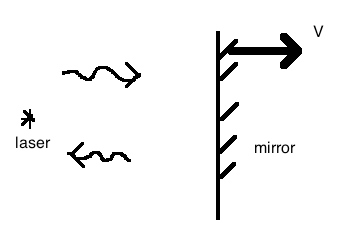
\includegraphics[width=0.35\textwidth]{images/mirror.png}
\caption{Mirror}
\end{figure}

\subsection{4-acceleration}
The definition $\vec{u}=\frac{d\vec{x}}{d\tau}$ is completely general in curved space. But acceleration is \underline{not} $\vec{a}=\frac{d\vec{u}}{d\tau}$ in general. This is because the 2nd derivative $\frac{d^2\vec{x}}{d\tau^2}$ cares about curvature (while the 1st derivative does not).

Actually: $\vec{a}=\nabla_{\vec{u}}\vec{u}$ in general.

In flat space: $\vec{a}=\frac{d\vec{u}}{d\tau}$, which is a special case.

\begin{equation}
\underbrace{\vec{u}\cdot\vec{u}=-1}_{\text{normalisation}}\Rightarrow \underbrace{\vec{u}\cdot\vec{a}=0}_{\text{differentiate both sides w.r.t $\tau$}}\label{4-accel diff}
\end{equation}
Equation (\ref{4-accel diff}) is true in curved space.

\hrule

Let's consider a case of \textbf{Uniform acceleration}. Consider a rocket ship with constant \emph{proper} acceleration $g$ in the ``1'' direction (achieved by, for example, throwing bricks out the back of the rocket at a constant rate), in flat spacetime.

In momentarily comoving reference frame:
\begin{align*}
g&=(-1,1,1,1)\\
\vec{u}&=(1,0,0,0)\\
\vec{a}&=(0,\frac{d^2\vec{x}}{d\tau^2},0,0)
\end{align*}
Above, $a^0$ is zero because
\begin{equation}
-a^t=\vec{u}\cdot\vec{a}=0
\end{equation}
and $a^1$ is equal to $g$ by definition. Hence $\vec{a}\cdot\vec{a}=g^2$. This invariant $\Rightarrow$ true in all coordinates, but ONLY true in \emph{flat spacetime}.

Now consider motion in global Minkowski coordinates not tied to the rocket (which exists because spacetime is flat).

We want to solve for $u^0(\tau),u^1(\tau),a^0(\tau),a^1(\tau)$ in general.
\begin{align*}
\vec{u}\cdot\vec{u}&=-1&-(u^0)^2+(u^1)^2&=-1\\
\vec{a}\cdot\vec{u}&=0& -a^0 u^0+u^1 a^1&=0 \\
\vec{a}\cdot\vec{a}&=g^2& -(a^0)^2+(a^1)^2&=g^2
\end{align*}
Eliminating variables and solving (using straightforward algebra), we obtain 
\begin{align*}
\frac{du^0}{d\tau}&=a^0=gu^1\\
\frac{du^1}{d\tau}&=a^1=gu^0
\end{align*}
Integrating these gives
\begin{align*}
t&=\frac{1}{g}\sinh g\tau\\
x&=\frac{1}{g}\cosh g\tau
\end{align*}

\begin{figure}[h]
\centering
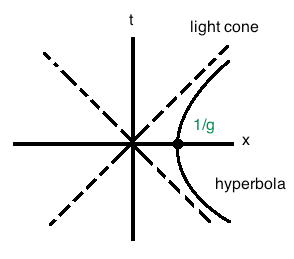
\includegraphics[width=0.3\textwidth]{images/rocket_hyperbola.png}
\caption{Rocket hyperbola}
\end{figure}

Remember this is in \emph{flat spacetime} The interesting thing about this diagram is that is shows that ANY photon more than $1/g$ distance away from the rocket ship at $t=0$ will never reach the rocket ship, even though the rocket ship is travelling less than $c$.


\section{Calculus in curved space}

\subsection{Differentiation in curved space}
Covariant derivatives $\to$ curvature $\to$ Einstein's field equations. Curvature is the second order change in space.

How does a tensor $T$ of type $\pmx{M\\N}$ change from spacetime point $P_A$ to $P_B$? (we consider these points to be infinitesimally separated).

\begin{figure}[h]
\centering
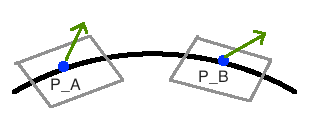
\includegraphics[width=0.5\textwidth]{images/tangent-spaces.png}
\caption{Tangent spaces}
\end{figure}

In general, we cannot compare geometric objects at $P_A$ and $P_B$ (they live in different tangent spaces) unless we have a recipe for ``moving'' geometric objects from $P_A$ to $P_B$, e.g. parallel transport (which we will consider later).

For now we just consider \underline{flat} space, where all points share a common tangent space.


Look for $\pmx{M\\N+1}$ tensor $\nabla T$ which contracts with a vector $\vec{A}$ to give infinitesimal rate of change of $T$ along $\vec{A}$. We call the rate of change $\nabla_{\vec{A}}T$ (type $\pmx{M\\N}$) the \emph{covariant derivative}
\begin{equation}
\nabla_{\vec{A}} T=\langle \nabla T,\vec{A}\rangle
\end{equation}

e.g. if $T$ is a scalar $\underbrace{\phi}_{\pmx{0\\0}\text{ type}}$, then $\nabla T=\underbrace{\tilde{d\phi}}_{\text{gradient }\pmx{0\\1}}$

e.g. if T is a vector, say $\vec{V}$: in general consider two points $P_A$, $P_B$ joined by a world line $\vec{x}(t)$

\begin{figure}[h]
\centering
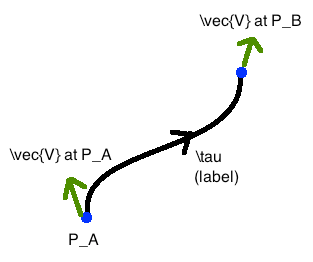
\includegraphics[width=0.5\textwidth]{images/world-line.png}
\caption{World line connecting points $P_A$ and $P_B$}
\end{figure}

\begin{align*}
\frac{d\vec{V}}{d\tau}(\vec{x}(\tau))&=\frac{d}{d\tau}\left[V^{\alpha}(\vec{x}(\tau))\vec{e}_{\alpha}
(\vec{x}(\tau))\right]\\
&=\frac{\partial V^{\alpha}}{\partial x^{\beta}}\frac{dx^{\beta}}{d\tau}\vec{e}_{\alpha}(\vec{x}(\tau))
+V^{\alpha}\frac{\partial \vec{e}_{\alpha}}{\partial x^{\beta}}\frac{dx^{\beta}}{d\tau}\qquad\text{product rule}\\
&=\left(\frac{\partial V^{\alpha}}{dx^{\beta}}\vec{e}_{\alpha}+V^{\alpha}\frac{\partial \vec{e}_{\alpha}}{\partial x^{\beta}}\right)u^{\beta}\qquad\text{4-velocity}\label{diff eqn1}
\end{align*}

The parts inside the brackets of (\ref{diff eqn1}), denoted as $(\ldots)$, are contracted with $\vec{u}$ to give the LHS, which is a vector. So $(\ldots)$ is type $\pmx{1\\1}$.

$\frac{\partial \vec{e}_{\alpha}}{\partial x^{\beta}}$ are vectors, so can be written as a linear combination of basis vectors. 

\begin{equation}
\text{Define: } \frac{\partial \vec{e}_{\alpha}}{\partial x^{\beta}}=\Gamma^{\mu}_{\alpha\beta} \vec{e}_{\mu}\label{de dx with chris}
\end{equation}

Then,

\begin{align*}
(\ldots)&=\frac{\partial V^{\alpha}}{\partial x^{\beta}}\vec{e}_{\alpha} + V^{\alpha}\Gamma^{\mu}_{\alpha\beta}\vec{e}_{\mu}\\
&=\left(\frac{\partial V^{\alpha}}{\partial x^{\beta}}+\Gamma^{\alpha}_{\mu\beta}V^{\mu}\right)
\vec{e}_{\alpha}
\end{align*}

The bracketed part above is, in index notation, $V^{\alpha}_{; \beta}$; the components of covariant derivation $\nabla \vec{V}$ of type $\pmx{1\\1}$.

Notation: switch $\mu \leftrightarrow \alpha$ in \underline{dummy} index (repeated).

Christoffel symbols $\Gamma$:
\begin{itemize}
\item $4\times 4\times 4=64$ numbers
\item solve 64 equations given by (\ref{de dx with chris}) - linear equations (easy to solve!)
\begin{itemize}
\item an alternative trick is to use the metric, which we will see later
\end{itemize}
\item are Christoffel symbols components of a $\pmx{1\\2}$ tensor?
\begin{itemize}
\item No!
\item $\{\Gamma^{\mu}_{\alpha\beta}\vec{e}_{\mu}\}$ are components of a tensor, but the $\Gamma$'s themselves are not
\item e.g. is $\Gamma$'s are tensor, then
\begin{equation}
\Gamma^{\mu'}_{\alpha' \beta'}=\frac{\partial x^{\mu'}}{\partial x^{\mu}}\frac{\partial x^{\alpha}}{\partial x^{\alpha'}}\frac{\partial x^{\beta}}{\partial x^{\beta'}}\Gamma^{\mu}_{\alpha\beta}\label{tensor Chris}
\end{equation}
\item but from the definition of $\Gamma$'s we have $\Gamma^{\mu}_{\alpha\beta}=0$ for (say) Cartesian coordinates, which would then wrongly imply $\Gamma^{\mu'}_{\alpha'\beta'}$ from (\ref{tensor Chris}) too!
\end{itemize}
\end{itemize}

Physically: suppose you have a vector $\vec{V}$ which does \underline{not} change from point to point. We want $\nabla \vec{V}=0$.

\begin{figure}[h]
\centering
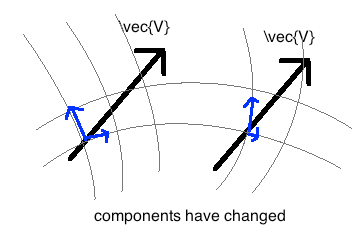
\includegraphics[width=0.5\textwidth]{images/vectors-v.png}
\caption{Vectors V}
\label{Christoffel image}
\end{figure}

If the coordinates are curvilinear, then components ``artificially'' change. The $\Gamma$'s ``undo'' the artificial change!


\review{
\begin{align*}
T&=\pmx{M\\N}\text{ tensor}\\
\nabla T&=\pmx{M\\N+1}\text{ tensor}\\
\nabla_{\vec{A}}T&=\text{covariant derivative of T along }\vec{A}=\langle\nabla T,\vec{A}\rangle=\text{type }\pmx{M\\N}
\end{align*}

e.g. if $T$ of a scalar $\phi$ then $\nabla T=\tilde{d\phi}$

e.g. if $T$ is a vector $\vec{V}$ then $\nabla \vec{V}$ is a $\pmx{1\\1}$ object
\begin{equation}
\underbrace{(\nabla \vec{V})^{\alpha}_{\beta}}_{\text{notation: }V^{\alpha}_{;\beta}}=
\underbrace{\frac{\partial V^{\alpha}}{\partial x^{\beta}}}_{\text{notation: }V^{\alpha}_{,\beta}}
+\underbrace{\Gamma^{\alpha}_{\lambda\beta}}_{\text{Christoffel}}V^{\lambda}
\end{equation}

Christoffel symbol corrects for artificial change in components of $\vec{V}$ due to curvilinear coordinates (see Figure \ref{Christoffel image}). Derived for curvilinear coordinates in flat space but remains true for curved spaces also!

\underline{Note:} neither $V^{\alpha}_{,\beta}$ nor $\Gamma^{\mu}_{\alpha\beta}$ are tensors ($\Gamma$'s are components of set of tensors $\{\nabla \vec{e}_{\alpha}\}$). But $V^{\alpha}_{;\beta}$
}

\subsection{Covariant derivative of 1-form}
What about 1-forms? Can we just say

\begin{equation*}
p_{\alpha;\beta}=\frac{\partial p_{\alpha}}{\partial x^{\beta}}
+\Gamma^{\alpha}_{\lambda\beta}p_{\lambda}\quad \text{??}
\end{equation*}

No, we cannot - note the double lowered $\lambda$ in the RHS.

$\nabla\tilde{p}$ is $\pmx{0\\2}$ type/

We redo rate-of-change calculation along world line $\vec{x}$
\begin{align}
\frac{d\tilde{p}}{d\tau}&=\frac{d}{d\tau}\left[p_{\alpha}(\vec{x}(\tau))\tilde{\omega}^{\alpha}(\vec{x}(\tau))\right]\\
&=\frac{\partial p_{\alpha}}{dx^{\beta}}\frac{dx^{\beta}}{d\tau}\tilde{\omega}^{\alpha}+p_{\alpha}\underbrace{\frac{\partial \tilde{\omega}^{\alpha}}{\partial x^{\beta}}}_{\text{1-form}}
\frac{dx^{\beta}}{d\tau}
\end{align}

We can write the 1-form as linear combination $x_{\mu\beta}^{\alpha}\tilde{\omega}^{\mu}$

Are $x$'s related to $\Gamma$;s? Yes - duality.
\begin{equation}
\delta ^{\alpha}_{\beta}=\langle \tilde{\omega}^{\alpha},\vec{e}_{\beta}\rangle\qquad \text{from previous lectures}
\end{equation}

Differentiate by $x^{\gamma}$
\begin{align}
0&=\langle\frac{\partial\tilde{\omega}^{\alpha}}{\partial x^{\gamma}},\vec{e}_{\beta}\rangle 
\langle \tilde{\omega}^{\alpha},\frac{\partial \vec{e}_{\beta}}{\partial x^{\gamma}}\\
&=\langle x_{\mu\gamma}^{\alpha}\tilde{\omega}^{\mu},\vec{e}_{\beta}\rangle +\langle\tilde{\omega}^{\alpha},\Gamma^{\lambda}_{\beta\gamma}\vec{e}_{\lambda}\rangle\\
&=x^{\alpha}_{\mu\gamma}\delta^{\mu}_{\beta}
+\Gamma^{\lambda}_{\beta\gamma}\delta^{\alpha}_{\lambda}\\
&=x^{\alpha}_{\beta\gamma}+\Gamma^{\alpha}_{\beta\gamma}
\end{align}
i.e. opposites!

Components of $\nabla\tilde{p}$, i.e. $(\nabla\tilde{p})_{\alpha\beta}$ is notationally $p_{\alpha;\beta}$

\begin{equation}
p_{\alpha;\beta}=\frac{\partial_{\alpha}}{\partial x^{\beta}}-\Gamma^{\lambda}_{\alpha\beta} p_{\lambda}
\end{equation}

For general tensor: add correction term $\pm \Gamma$ tensor for each tensor index; $+$ is index is up; $-$ if index is down.

\begin{equation}
\text{e.g. } T^{\alpha}_{\beta;\gamma}=\frac{\partial T^{\alpha}_{\beta}}{\partial^{\gamma}}
+\underbrace{\Gamma^{\alpha}_{\lambda\gamma} T^{\lambda}_{\beta}}_{\text{by analogy with vector}}
-\underbrace{\Gamma^{\lambda}_{\beta \gamma}T^{\alpha}_{\lambda}}_{\text{by analogy with 1-form}}
\end{equation}

\subsection{Covariant derivative of metric}

Recall
\begin{align}
\nabla \vec{V}&=\pmx{1\\1}\text{ type}\\
\nabla \tilde{V}&=\pmx{0\\2}\text{ type}
\end{align}
where $\tilde{V}$ is the specific 1-form induced by the metric with $\vec{V}$ in the one slot ($\tilde{V}=g(\vec{V},\ldots)$).

We can go from $\pmx{0\\2}$ to $\pmx{1\\1}$ by contraction! 

Consider $\nabla_{\vec{a}}\vec{V}=\pmx{1\\0}$ object. 

Then $g(\nabla_{\vec{A}}\vec{V},\ldots)$ is a 1-form induced by $g$. 

By definition this is $\nabla_{\vec{A}}\tilde{V}$ which is a 1-form, i.e. $\nabla\tilde{V}\pmx{0\\2}$ contracted with $\vec{A}$. 

In index notation:
\begin{equation}
V_{\alpha;\beta}=g_{\alpha\gamma}V^{\gamma}_{;\beta}\qquad\text{as in previous lectures}
\end{equation}


\subsection{Christoffel Symbols and Metric and Acceleration}
\subsubsection{Covariant derivative}
$\nabla g$ is a $\pmx{0\\3}$ tensor (with components $g_{\alpha\beta ; \gamma}$).

From last time, given $\vec{V}$ there is a $\tilde{V}$.

By definition,
\begin{equation}
V_{\alpha;\beta}=g_{\alpha\gamma} V^{\gamma}_{;\beta}\quad\text{(or $\nabla_{\vec{A}}\vec{V}$)}\label{product rule}
\end{equation}

Separately,
\begin{equation}
V_{\alpha}=g_{\alpha\beta}V^{\gamma}\label{Valph}
\end{equation}

Taking the covariant derivative of both sides of (\ref{Valph}) with respect to $x^{\beta}$
\begin{align}
\Rightarrow V_{\alpha;\beta}&=g_{\alpha\gamma;\beta}V^{\gamma}+g_{\alpha\gamma}V^{\gamma}_{;\beta}\\
&\Rightarrow g_{\alpha\gamma;\beta=0}\\
&\Rightarrow \nabla g=0
\end{align}

We can use this to get a formula for $\Gamma$'s ($\Gamma$'s are coefficients in linear combination of basis vectors which give $\frac{\partial \vec{e}_{\alpha}}{\partial x_{\beta}}$)

An alternative derivation of $\nabla g=0$:

In flat space, $g_{\alpha\beta , \gamma}=0$ \underline{and} $\Gamma$'s are zero because $\frac{\partial\vec{e}_{\alpha}}{\partial x^{\beta}}=0$
\begin{align}
\Rightarrow g_{\alpha\beta;\gamma}&=g_{\alpha\beta,\gamma}-(\text{two terms involving Christoffel symbols})\\
&=0 \quad\text{in flat space}
\end{align}

But $g_{\alpha\beta;\gamma}=0$ involves only decent tensors, so it's free in ????

\begin{equation}
-=g_{\alpha\beta;\gamma}=g_{\alpha\beta,\gamma}-\Gamma^{\lambda}_{\alpha\gamma}g_{\lambda\beta}
\end{equation}

??? gives us 64 equations for 64 unknowns ($\Gamma$ components) provided $g_{\alpha\beta}$ and $g_{\alpha\beta,\gamma}$ are given.

Simplification: symmetric in $\alpha,\beta$; symmetric in lower indices of the $\Gamma$'s

Using this and write three cyclic permutations of (*) and sum them (see Schutz p. 142):

\begin{equation}
\Gamma^{\lambda}_{\alpha\beta}=\frac{1}{2}g^{\lambda\mu}(g_{\mu\alpha,\beta}+g_{\mu\beta,\alpha}-g_{\alpha\beta,\mu})\label{chris to mem}
\end{equation}
You should memorise equation (\ref{chris to mem})!

\begin{itemize}
\item If Minkowski:
\begin{itemize}
\item $\Gamma$'s are 0
\end{itemize}
\item If not:
\begin{itemize}
\item $\Gamma\text{'s}\neq 0$, coordinates are curved, but space may not be curved
\end{itemize}
\end{itemize}

Curvatures of manifold depend on 2nd derivatives of g.

\subsection{The 4-acceleration}
$\vec{u}=\frac{d\vec{x}}{d\tau}$ is a first derivative (i.e. this is calculated without reference to curvature of coordinates and/or manifold).

$\vec{a}$ is a second derivative. We need to refer to curvature of coordinates/manifold.

In general, $\vec{a}=\nabla_{\vec{u}}\vec{u}$, i.e. rate of change of $\vec{i}$ along itself.

In free fall: $\nabla_{\vec{u}}\vec{u}=0$ (but with rocket engines $\nabla_{\vec{u}}\vec{u}\neq 0$)

Christoffel symbols contain curvature!

\review{Last lecture: \begin{itemize}
\item $\Gamma^{\lambda}_{\alpha\beta}=\frac{1}{2}g^{\lambda\mu}(g_{\mu\alpha,\beta}+g_{\mu\beta,\alpha}-g_{\alpha\beta,\mu})$
\item $g_{\alpha\beta;\gamma}=0$
\end{itemize}
}

Remember, for curved space, 4-acceleration $\vec{a}\neq\frac{d^2\vec{x}}{d\tau^2}$. This is the derivative of $x^{\alpha}(\vec{e}_{\alpha})$ not just coordinates. $\tau$ involves curvature.

For free fall, $\vec{a}=0$ (compare with Newtonian $\SI{9.8}{ms^{-2}}$

\example{?}{Astronaut above Schwarz. black hole, at distance $r$ (radial coordinate appearing in metric), with $\theta$ and $\phi$ also fixed. The Schwarzchild metric is:
\begin{align}
g_{tt}&=-\left(1-\frac{2M}{r}\right)\\
g_{rr}&=\left(1-\frac{2M}{r}\right)^{-1}\\
g_{\theta\theta}&=...\\
g_{\phi\phi}&=...
\end{align}

Note: rotating black hole is not diagonal! (but it will be symmetric because $A^{\alpha}\vec{e}_{\alpha}=A^{\beta}\vec{e}_{\beta}$; non-diagonal $\Leftarrow$ diagonal (one way!))

Question: what is the acceleration of this astronaut (globally not flat) at a fixed radius?

We need $\vec{u}=\left(\frac{dt}{d\tau},0,0,0\right)$

\begin{align}
\vec{x}&=(t,r,\theta,\phi)\\
\vec{u}&=\frac{d\vec{x}}{d\tau}
\end{align}

What is $u_t$? We need to normalise.

\begin{align}
\vec{u}\cdot\vec{u}&=-1\\
u^\beta g^{\alpha\beta}u_{\alpha}&=-\left(1-\frac{2M}{r}\right)=u_t^2=-1\\
&\Rightarrow u_t=\left(1-\frac{2M}{r}\right)^{-1/2}
\end{align}

\begin{align}
a^{\alpha}&=u^{\beta}u^{\alpha}_{;\beta}\quad\text{covariant derivative}\\
&=u^{\beta}\left(\frac{\partial u^{\alpha}}{\partial x^{\beta}}+\Gamma^{\alpha}_{\lambda\beta}u^{\lambda}\right)\\
&=\underbrace{\frac{\partial u^{\alpha}}{\partial\tau}}_{\text{zero}}+\Gamma^{\alpha}_{\lambda\beta}u^{\lambda}u^{\beta}
\end{align}

Now,
\begin{align}
a^t=a^{\theta}=a^{\phi}&=0\\
\Rightarrow a^{r}&=\Gamma^{r}_{tt}(u^t)^2\\
&=\frac{M}{r^2}\left(1-\frac{2M}{r}\right)\cdot\left[\left(1-\frac{2M}{r}\right)^{-1/2}\right]^2=\frac{M}{r^2}
\end{align}

\begin{equation}
\vec{a}=\nabla_{\vec{u}}\vec{u}=(0,\frac{M}{r^2},0,0)=\frac{M}{r^2}\hat{r}\quad\text{(accelerating outwards!)}
\end{equation}

We will prove that acceleration is always orthogonal to the 4-velocity.

\begin{align}
\vec{u}\cdot\vec{u}&=-1=u^{\alpha}u_{\alpha}
\intertext{Take the covariant derivative}
\Rightarrow 0&=(u^{\alpha}_{;\beta}u_{\alpha}+u^{\alpha}u_{\alpha;\beta})u^{\beta}\\
&=(u^{\alpha}_{;\beta}u_{\alpha}+u_{\gamma}g^{\gamma\alpha}u_{\alpha;\beta})u^{\beta}\quad\text{(note $g^{\gamma\alpha}_{;\beta}=0$)}\\
0&=(u^{\alpha}_{;\beta}u_{\alpha}+u_{\gamma}u^{\gamma}_{;\beta})u^{\beta}
\end{align}
where we have switched co- and contra-variant indices using the metric!

So $(u_\alpha u^{\alpha}_{;\beta})u^{\beta}=0$ (both terms are equal).
\begin{equation}
\Rightarrow \vec{u}\cdot\vec{a}=0
\end{equation}
}


\subsection{Fermi-Walker Transport}

What does the ``natural basis'' of an observer in a rocket ship $(\vec{a},\vec{v})$ in curved space look like, compared to some external basis? (global coordinate system)

We let $\vec{v}$ be an arbitrary vector. We then solve
\begin{equation}
\nabla_{\vec{u}}\vec{v}=(\vec{a}\cdot\vec{v})\vec{u}-\vec{a}(\vec{u}\cdot\vec{v})
\end{equation}
to see what $\vec{v}$ and $\vec{u}$ look like in a global coordinate system.

Not unique apparently. However,
\begin{enumerate}
\item 
\begin{equation}
\nabla_{\vec{u}}(\vec{v}\cdot\vec{v})=2\vec{v}\cdot\nabla_{\vec{u}}\vec{v}=0\quad\text{lengths preserved}
\end{equation}
\item 
\begin{equation}
\nabla_{\vec{u}}(\vec{v}\cdot\vec{w})=\vec{v}\cdot\nabla_{\vec{u}}\vec{w}+\vec{w}\cdot\nabla_{\vec{u}}\vec{v}=0
\quad\text{angles preserved (orthogonality)}
\end{equation}
\item
4-velocity is Fermi-Walker transported automatically. (if $\vec{v}=\vec{u}$ then
\begin{align}
\nabla_{\vec{u}}\vec{v}&=(\vec{a}\cdot\vec{u})\vec{u}-\vec{a}(\vec{u}\cdot\vec{u})\\
&=\vec{a}\quad\text{identically satisfied}
\end{align}
You can treat your time axis to be $\vec{u}$ (along the path).
\item
If $\vec{w}$ is spacelike (orthogonal to $\vec{a}$ and $\vec{u}$), then $\nabla_{\vec{u}}\vec{w}=0$ ($\vec{w}$ does not rotate spatially relative to $\vec{u}$) (it's temporal (?))
\end{enumerate}

\subsection{Constants of motion}

Approach \#1: use Lagrangian methods

Approach \#2: for free fall
\begin{equation}
\nabla_{\vec{u}}\vec{u}=0 \label{freefall crit}
\end{equation}
(for a photon $\nabla_{\vec{p}}\vec{p}=0$)
We can also look at the 1-form version of equation (\ref{freefall crit})
\begin{equation}
\nabla_{\vec{u}}\tilde{u}=0
\end{equation}
\begin{align}
\text{Components: }\quad&u^{\beta}_{\alpha;\beta}=0\\
&\underbrace{u^{\beta}}_{=\frac{\partial x^{\beta}}{d\tau}}
\left(\frac{\partial u_{\alpha}}{\partial x^{\beta}}-\Gamma^{\lambda}_{\alpha\beta}u^{\lambda}\right)=0
\end{align}

\begin{equation}
\text{i.e., } \underbrace{\frac{\partial u_{\alpha}}{d\tau}}_{\text{chain rule}}
=\Gamma^{\lambda}_{\alpha\beta}u_{\lambda}u^{\beta}
\end{equation}

\begin{align}
\text{Recall: }\quad&&\Gamma^{\lambda}_{\alpha\beta}&=\frac{1}{2}g^{\lambda\mu}
(g_{\mu\alpha,\beta}+g_{\mu\beta,\alpha}-g_{\alpha\beta,\mu})\\
&&\Gamma^{\lambda}_{\alpha\beta}u_{\lambda}u^{\beta}
&=\frac{1}{2}\underbrace{u^{\mu}u^{\beta}}_{\text{symm. }\mu\leftrightarrow \beta}
(g_{\mu\alpha,\beta}+g_{\mu\beta,\alpha}-g_{\alpha\beta,\mu})
\intertext{Now, $g_{\mu\alpha,\beta}$ and $g_{\alpha\beta,\mu}$ are antisymmetric under exchange of $\mu\leftrightarrow\beta$}
&&&=\frac{1}{2}u^{\mu}u^{\beta}g_{\mu\beta,\alpha}
\end{align}
since contraction of symmetric and antisymmetric components vanishes.

i.e., if the metric is independent of coordinate $x^{\alpha}$ then $u_{\alpha}$ is constant along world line.

e.g., in Schwarz spacetime, a freely falling body has $u_{\phi}=\text{constant}$ and $u_t=\text{constant}$.


\subsection{Polar coordinates}

We shall explore polar coordinates through use of an example.

Polar coordinates (primed): $(r,\theta)$

Cartesian (unprimed): $(x,y)$
\begin{align}
x&=r\cos\theta\\
y&=r\sin\theta
\end{align}

Our plan is:
\begin{itemize}
\item get polar basis
\item get polar metric
\item get polar Christoffel symbol
\end{itemize}

To get \textbf{polar basis}:

Transformation matrix:
\begin{align}
\frac{\partial x^{\alpha}}{\partial x^{\alpha'}}&=\pmx{\frac{\partial x}{\partial r}&\frac{\partial x}{\partial \theta}\\
\frac{\partial y}{\partial r}&\frac{\partial y}{\partial \theta}}=\pmx{\cos\theta&-r\sin\theta\\\sin\theta&r\cos\theta}\\
\frac{\partial x^{\alpha'}}{\partial x^{\alpha}}&=\pmx{\frac{\partial r}{\partial x}&\frac{\partial r}{\partial y}\\
\frac{\partial \theta}{\partial x}&\frac{\partial \theta}{\partial y}}=\ldots \quad\text{exercise}
\end{align}


Basis vectors:
\begin{align}
\vec{e}_{\alpha}&=\frac{\partial x^{\alpha'}}{\partial x^{\alpha}}\vec{e}_{\alpha'}\\
\vec{e}_r&=\frac{\partial x}{\partial r}\vec{e}_x+\frac{\partial y}{\partial r}\vec{e}_y\\
&=\cos\theta\vec{e}_x+\sin\theta\vec{e}_y\\
\vec{e}_{\theta}&=\frac{\partial x}{\partial \theta}\vec{e}_x+\frac{\partial y}{\partial \theta}\vec{e}_y\\
&=-r\sin\theta\vec{e}_x+r\cos\theta \vec{e}_y
\end{align}

\begin{center}[h]

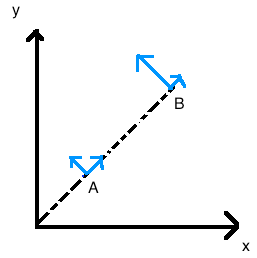
\includegraphics[width=0.5\textwidth]{images/polar.png}
\captionof{figure}{Polar coordinates?}
\label{polar coords fig}
\end{center}
 
In Figure \ref{polar coords fig} above we see the vector length at $B$ is greater than at $A$; the length of $\vec{e}_\theta$ is proportional to $r$ because we need to subtend a greater arc further out so as to produce unit change in $\theta$.


\textbf{Polar metric}:
\begin{align}
g_{\alpha'\beta'}&=\vec{e}_{\alpha'}\vec{\beta'}\\
g_{rr}&=\vec{e}_r\cdot\vec{e}_r=1\\
g_{r\theta}&=\vec{e}_r\cdot \vec{e}_{\theta}=0\\
g_{\theta\theta}&=\vec{e}_{\theta}\cdot\vec{e}_{\theta}=r^2
\end{align}

\exercise{
Check this this also follows from the transformation law
\begin{equation}
g_{\alpha'\beta'}=\frac{\partial x^{\alpha}}{\partial x^{\alpha'}}\frac{\partial x^{\beta}}{\partial x^{\beta'}}
\underbrace{g_{\alpha\beta}}_{\pmx{1&0\\0&1}\text{ Cartesian}}
\end{equation}
}
{}

Christoffel symbols describe derivatives of basis vectors in that basis itself

\begin{align}
\frac{\partial \vec{e}_r}{\partial r}&=0\\
\frac{\partial \vec{e}_r}{\partial \theta}&=-\sin\theta\vec{e}_x+\cos\theta \vec{e}_y\\
\frac{\partial \vec{e}_{\theta}}{\partial r}&=-\sin\theta\vec{e}_x+\cos\theta\vec{e}_y\\
\frac{\partial \vec{e}_{\theta}}{\partial \theta}&=-r\cos\theta \vec{e}_x-r\sin\theta\vec{e}_y
\end{align}

Expressing these in the basis we get
\begin{center}
\begin{tabular}{l|l|l}
$\frac{\partial \vec{e}_r}{\partial r}=0$ & $\Gamma^{r}_{rr}=0$&$\Gamma^{\theta}_{rr}=0$\\
$\frac{\partial \vec{e}_r}{\partial \theta}=\frac{1}{r}\vec{e}_\theta$ & $\Gamma^{r}_{r\theta}=0$&$\Gamma^{\theta}_{r\theta}=\frac{1}{r}$\\
$\frac{\partial \vec{e}_{\theta}}{\partial r}=\frac{1}{r}\vec{e}_{\theta}$ & $\Gamma^{r}_{\theta r}=0$&$\Gamma^{\theta}_{\theta r}=\frac{1}{r}$\\
$\frac{\partial \vec{e}_{\theta}}{\partial \theta}=-r\vec{e}_r$ & $\Gamma^{r}_{\theta\theta}=-r$&$\Gamma^{\theta}_{\theta \theta}=0$\\
\end{tabular}
\end{center}

Important to recall:
\begin{equation}
\frac{\partial \vec{e}_{\alpha}}{\partial x^{\beta}}=\vec{e}_{\mu}\Gamma^{\mu}_{\alpha\beta}
\end{equation}

We should check this works when taking covariant derivative of $\vec{V}$.

Special case: $\vec{V}=\vec{e}_{x}=\text{constant}$. We should find $\nabla_{\vec{A}}\vec{V}=0$ for all $\vec{A}$.

To check: we write $\vec{V}$ in polar coordinates:
\begin{equation}
\vec{V}=\cos\theta\vec{e}_{r}-\frac{1}{r}\sin\theta\vec{e}_{\theta}
\end{equation}
from transformation laws for basis vectors.

\begin{align*}
\left(\nabla_{\vec{A}}\vec{V}\right)^{\alpha}&=A^{\beta}\left(\frac{\partial V^{\alpha}}{\partial x^{\beta}}+\Gamma^{\alpha}_{\lambda\beta}V^{\lambda}\right)\\
\therefore \left(\nabla_{\vec{A}}\vec{V}\right)^{r}&=A^{\beta}\frac{\partial V^{r}}{\partial x^{\beta}}+\Gamma^r_{\lambda\beta}V^{\lambda}A^{\beta}\\
&=A^{\theta}\frac{\partial V^r}{\partial \theta}+\Gamma^{r}_{\theta\theta}V^{\theta}A^{\theta}\quad\text{other terms zero}\\
&=A^{\theta}(-\sin\theta)-r\cdot\left(-\frac{1}{r}\sin\theta\right)A^{\theta}\\
&=0\\
\left(\nabla_{\vec{A}}\vec{V}\right)^{\theta}&=A^{\beta}\frac{\partial V^{\theta}}{\partial x^{\beta}}+\Gamma^{\theta}_{\lambda\beta}V^{\lambda}A^{\beta}\\
&=A^r\frac{\partial V^{\theta}}{\partial r}+A^{\theta}\frac{\partial V^{\theta}}{\partial \theta}+\Gamma^{\theta}_{r\theta}V^{r}A^{\theta}+\Gamma^{\theta}_{\theta r}V^{\theta}A^{r}\\
&=A^{r}\cdot\frac{1}{r^2}\sin\theta+A{\theta}\cdot\left(-\frac{\cos\theta}{r}\right)+\frac{1}{r}\cdot\cos\theta\cdot A^{\theta}+\frac{1}{r}\left(-\frac{1}{r}\sin\theta\right)A^r\\
&=0
\end{align*}

\exercise{Metric $g=\text{diag}(1,r^2)$ from previous lecture; check that $\nabla g=0$ explicitly.}{}

\exercise{Confirm that $\Gamma$'s can also be derived from
\begin{equation}
\Gamma^{\mu}_{\alpha\beta}=\frac{1}{2}g^{\mu\lambda}(g_{\lambda\alpha,\beta}+g_{\lambda\beta,\alpha}
-g_{\alpha\beta,\lambda})
\end{equation}}{}

\exercise{Prove divergence
\begin{equation}
V^{\alpha}_{;\alpha}=\frac{1}{r}\frac{\partial}{\partial r}(rV_r)+\frac{\partial V_{\theta}}{\partial \theta}
\end{equation}
as you would expect from undergrad.}{}

\exercise{Derive $\chi^{\mu}_{\alpha\beta}$'s for basis one-forms
\begin{align}
\tilde{\omega}^r&=\cos\theta\cdot\tilde{\omega}^x+\sin\theta\cdot\tilde{\omega}^y\\
\tilde{\omega}^{\theta}&=-\frac{\sin\theta}{r}\cdot\tilde{\omega}^x+\frac{\cos\theta}{r}\cdot\tilde{\omega}^y
\end{align}}{}


\section{Curved space}

In the presence of gravity, we cannot have a global inertial (Minkowski) frame.

\begin{figure}[h]
\centering
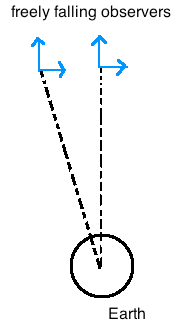
\includegraphics[height=0.2\textheight]{images/freely-falling-observers.png}
\caption{Freely falling observers}
\end{figure}
We see that the distance between the observers decreases! i.e. curved geodesics $\Rightarrow$ curved space!

\subsection{Curved manifold}
\begin{itemize}
\item Extrinsic curvature: is space curved with respect to the space in which it's embedded?
\begin{figure}[h]
\centering
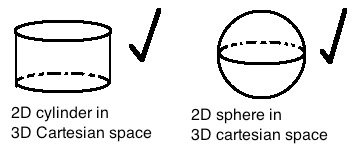
\includegraphics[width=0.5\textwidth]{images/extrinsic-curvature.png}
\caption{Extrinsic curvature}
\end{figure}\\
Yes!
\item Intrinsic curvature: without refernce to an emedding. Do neighbouring geodesics (``free fall'') diverge/converge? Note we need the idea of parallel transport to discuss geodesics.
\begin{figure}[h]
\centering
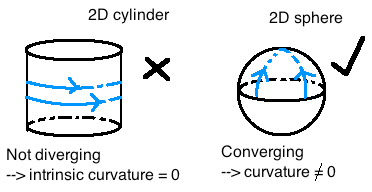
\includegraphics[width=0.5\textwidth]{images/intrinsic-curvature.png}
\caption{Intrinsic curvature}
\end{figure}\\
We see that a 2D cylinder does \underline{not} have intrinsic curvature!
\end{itemize}


\pagebreak



Indices up = vector-like

Indices down = 1-form-like

%-----------------------------------------
\end{document}




%\begin{tikzpicture}[line width=0.7 pt, xscale = 3, yscale = 3]

%\draw [fermion] (0,0)--(1.5,0);
%	\node at (0.75,0.3) {$\tau$};

%\end{tikzpicture}



